\documentclass[a4paper,12pt]{report}

%%%%%%%%%%%%%%%%%%%%%%%%%%%%%%%%%
% PACKAGE IMPORTS
%%%%%%%%%%%%%%%%%%%%%%%%%%%%%%%%%
\usepackage[tmargin=2cm,rmargin=1in,lmargin=1in,margin=0.85in,bmargin=2cm,footskip=.2in]{geometry}
\usepackage[none]{hyphenat}
\usepackage{amsmath,amsfonts,amsthm,amssymb,mathtools}
\allowdisplaybreaks
\usepackage{undertilde}
\usepackage{xfrac}
\usepackage[makeroom]{cancel}
\usepackage{mathtools}
\usepackage{bookmark}
\usepackage{enumitem}
\usepackage{kbordermatrix}
\renewcommand{\kbldelim}{(} % Change left delimiter to (
\renewcommand{\kbrdelim}{)} % Change right delimiter to )
\usepackage{hyperref,theoremref}
\hypersetup{
	pdftitle={Assignment},
	colorlinks=true, linkcolor=doc!90,
	bookmarksnumbered=true,
	bookmarksopen=true
}
\usepackage[most,many,breakable]{tcolorbox}
\usepackage{xcolor}
\usepackage{varwidth}
\usepackage{varwidth}
\usepackage{etoolbox}
%\usepackage{authblk}
\usepackage{nameref}
\usepackage{multicol,array}
\usepackage{tikz-cd}
\usepackage[ruled,vlined,linesnumbered]{algorithm2e}
\usepackage{comment} % enables the use of multi-line comments (\ifx \fi) 
\usepackage{import}
\usepackage{xifthen}
\usepackage{pdfpages}
\usepackage{svg}
\usepackage{transparent}
\usepackage{pgfplots}
\pgfplotsset{compat=1.18}
\usetikzlibrary{calc}
\usetikzlibrary{graphs}
\usetikzlibrary{graphs.standard}
% \usetikzlibrary{graphdrawing}

\newcommand\mycommfont[1]{\footnotesize\ttfamily\textcolor{blue}{#1}}
\SetCommentSty{mycommfont}
\newcommand{\incfig}[1]{%
    \def\svgwidth{\columnwidth}
    \import{./figures/}{#1.pdf_tex}
}


\usepackage{tikzsymbols}
% \renewcommand\qedsymbol{$\Laughey$}

\definecolor{commentgreen}{RGB}{2,112,10}
%%
%% Julia definition (c) 2014 Jubobs
%%
\lstdefinelanguage{Julia}%
  {morekeywords={abstract,break,case,catch,const,continue,do,else,elseif,%
      end,export,false,for,function,immutable,import,importall,if,in,%
      macro,module,otherwise,quote,return,switch,true,try,type,typealias,%
      using,while},%
   sensitive=true,%
   alsoother={$},%
   morecomment=[l]\#,%
   morecomment=[n]{\#=}{=\#},%
   morestring=[s]{"}{"},%
   morestring=[m]{'}{'},%
}[keywords,comments,strings]%

\lstset{%
    language        	= Julia,
    basicstyle      	= \ttfamily,
    keywordstyle    	= \bfseries\color{blue},
    stringstyle     	= \color{magenta},
    commentstyle    	= \color{commentgreen},
    showstringspaces	= false,
		numbers						= left,
		tabsize						= 4,
}

\definecolor{stringyellow}{RGB}{227, 78, 48}
%% 
%% Shamelessly stolen from Vivi on Stackoverflow
%% https://tex.stackexchange.com/questions/75116/what-can-i-use-to-typeset-matlab-code-in-my-document
%%
\lstset{language=Matlab,%
    %basicstyle=\color{red},
    breaklines=true,%
    morekeywords={matlab2tikz},
		morekeywords={subtitle}
    keywordstyle=\color{blue},%
    morekeywords=[2]{1}, keywordstyle=[2]{\color{black}},
    identifierstyle=\color{black},%
    stringstyle=\color{stringyellow},
    commentstyle=\color{commentgreen},%
    showstringspaces=false,%without this there will be a symbol in the places where there is a space
    numbers=left,%
		firstnumber=1,
    % numberstyle={\tiny \color{black}},% size of the numbers
    % numbersep=9pt, % this defines how far the numbers are from the text
    emph=[1]{for,end,break},emphstyle=[1]\color{red}, %some words to emphasise
    %emph=[2]{word1,word2}, emphstyle=[2]{style},    
}

%% 
%% Shamelessly stolen from egreg on Stackoverflow
%% https://tex.stackexchange.com/questions/280681/how-to-have-multiple-lines-of-intertext-within-align-environment
%%
\newlength{\normalparindent}
\AtBeginDocument{\setlength{\normalparindent}{\parindent}}
\newcommand{\longintertext}[1]{%
  \intertext{%
    \parbox{\linewidth}{%
      \setlength{\parindent}{\normalparindent}
      \noindent#1%
    }%
  }%
}

%\usepackage{import}
%\usepackage{xifthen}
%\usepackage{pdfpages}
%\usepackage{transparent}

%%%%%%%%%%%%%%%%%%%%%%%%%%%%%%
% SELF MADE COLORS
%%%%%%%%%%%%%%%%%%%%%%%%%%%%%%
\definecolor{myg}{RGB}{56, 140, 70}
\definecolor{myb}{RGB}{45, 111, 177}
\definecolor{myr}{RGB}{199, 68, 64}
\definecolor{mytheorembg}{HTML}{F2F2F9}
\definecolor{mytheoremfr}{HTML}{00007B}
\definecolor{mylenmabg}{HTML}{FFFAF8}
\definecolor{mylenmafr}{HTML}{983b0f}
\definecolor{mypropbg}{HTML}{f2fbfc}
\definecolor{mypropfr}{HTML}{191971}
\definecolor{myexamplebg}{HTML}{F2FBF8}
\definecolor{myexamplefr}{HTML}{88D6D1}
\definecolor{myexampleti}{HTML}{2A7F7F}
\definecolor{mydefinitbg}{HTML}{E5E5FF}
\definecolor{mydefinitfr}{HTML}{3F3FA3}
\definecolor{notesgreen}{RGB}{0,162,0}
\definecolor{myp}{RGB}{197, 92, 212}
\definecolor{mygr}{HTML}{2C3338}
\definecolor{myred}{RGB}{127,0,0}
\definecolor{myyellow}{RGB}{169,121,69}
\definecolor{myexercisebg}{HTML}{F2FBF8}
\definecolor{myexercisefg}{HTML}{88D6D1}

%%%%%%%%%%%%%%%%%%%%%%%%%%%%
% TCOLORBOX SETUPS
%%%%%%%%%%%%%%%%%%%%%%%%%%%%
\setlength{\parindent}{0pt}

%================================
% THEOREM BOX
%================================
\tcbuselibrary{theorems,skins,hooks}
\newtcbtheorem[number within=section]{Theorem}{Theorem}
{%
	enhanced,
	breakable,
	colback = mytheorembg,
	frame hidden,
	boxrule = 0sp,
	borderline west = {2pt}{0pt}{mytheoremfr},
	sharp corners,
	detach title,
	before upper = \tcbtitle\par\smallskip,
	coltitle = mytheoremfr,
	fonttitle = \bfseries\sffamily,
	description font = \mdseries,
	separator sign none,
	segmentation style={solid, mytheoremfr},
}
{th}

\tcbuselibrary{theorems,skins,hooks}
\newtcbtheorem[number within=chapter]{theorem}{Theorem}
{%
	enhanced,
	breakable,
	colback = mytheorembg,
	frame hidden,
	boxrule = 0sp,
	borderline west = {2pt}{0pt}{mytheoremfr},
	sharp corners,
	detach title,
	before upper = \tcbtitle\par\smallskip,
	coltitle = mytheoremfr,
	fonttitle = \bfseries\sffamily,
	description font = \mdseries,
	separator sign none,
	segmentation style={solid, mytheoremfr},
}
{th}


\tcbuselibrary{theorems,skins,hooks}
\newtcolorbox{Theoremcon}
{%
	enhanced
	,breakable
	,colback = mytheorembg
	,frame hidden
	,boxrule = 0sp
	,borderline west = {2pt}{0pt}{mytheoremfr}
	,sharp corners
	,description font = \mdseries
	,separator sign none
}

%================================
% Corollery
%================================
\tcbuselibrary{theorems,skins,hooks}
\newtcbtheorem[number within=section]{Corollary}{Corollary}
{%
	enhanced
	,breakable
	,colback = myp!10
	,frame hidden
	,boxrule = 0sp
	,borderline west = {2pt}{0pt}{myp!85!black}
	,sharp corners
	,detach title
	,before upper = \tcbtitle\par\smallskip
	,coltitle = myp!85!black
	,fonttitle = \bfseries\sffamily
	,description font = \mdseries
	,separator sign none
	,segmentation style={solid, myp!85!black}
}
{th}
\tcbuselibrary{theorems,skins,hooks}
\newtcbtheorem[number within=chapter]{corollary}{Corollary}
{%
	enhanced
	,breakable
	,colback = myp!10
	,frame hidden
	,boxrule = 0sp
	,borderline west = {2pt}{0pt}{myp!85!black}
	,sharp corners
	,detach title
	,before upper = \tcbtitle\par\smallskip
	,coltitle = myp!85!black
	,fonttitle = \bfseries\sffamily
	,description font = \mdseries
	,separator sign none
	,segmentation style={solid, myp!85!black}
}
{th}

%================================
% LENMA
%================================
\tcbuselibrary{theorems,skins,hooks}
\newtcbtheorem[number within=section]{Lenma}{Lenma}
{%
	enhanced,
	breakable,
	colback = mylenmabg,
	frame hidden,
	boxrule = 0sp,
	borderline west = {2pt}{0pt}{mylenmafr},
	sharp corners,
	detach title,
	before upper = \tcbtitle\par\smallskip,
	coltitle = mylenmafr,
	fonttitle = \bfseries\sffamily,
	description font = \mdseries,
	separator sign none,
	segmentation style={solid, mylenmafr},
}
{th}

\tcbuselibrary{theorems,skins,hooks}
\newtcbtheorem[number within=chapter]{lenma}{Lenma}
{%
	enhanced,
	breakable,
	colback = mylenmabg,
	frame hidden,
	boxrule = 0sp,
	borderline west = {2pt}{0pt}{mylenmafr},
	sharp corners,
	detach title,
	before upper = \tcbtitle\par\smallskip,
	coltitle = mylenmafr,
	fonttitle = \bfseries\sffamily,
	description font = \mdseries,
	separator sign none,
	segmentation style={solid, mylenmafr},
}
{th}

%================================
% PROPOSITION
%================================
\tcbuselibrary{theorems,skins,hooks}
\newtcbtheorem[number within=section]{Prop}{Proposition}
{%
	enhanced,
	breakable,
	colback = mypropbg,
	frame hidden,
	boxrule = 0sp,
	borderline west = {2pt}{0pt}{mypropfr},
	sharp corners,
	detach title,
	before upper = \tcbtitle\par\smallskip,
	coltitle = mypropfr,
	fonttitle = \bfseries\sffamily,
	description font = \mdseries,
	separator sign none,
	segmentation style={solid, mypropfr},
}
{th}

\tcbuselibrary{theorems,skins,hooks}
\newtcbtheorem[number within=chapter]{prop}{Proposition}
{%
	enhanced,
	breakable,
	colback = mypropbg,
	frame hidden,
	boxrule = 0sp,
	borderline west = {2pt}{0pt}{mypropfr},
	sharp corners,
	detach title,
	before upper = \tcbtitle\par\smallskip,
	coltitle = mypropfr,
	fonttitle = \bfseries\sffamily,
	description font = \mdseries,
	separator sign none,
	segmentation style={solid, mypropfr},
}
{th}

%================================
% CLAIM
%================================
\tcbuselibrary{theorems,skins,hooks}
\newtcbtheorem[number within=section]{claim}{Claim}
{%
	enhanced
	,breakable
	,colback = myg!10
	,frame hidden
	,boxrule = 0sp
	,borderline west = {2pt}{0pt}{myg}
	,sharp corners
	,detach title
	,before upper = \tcbtitle\par\smallskip
	,coltitle = myg!85!black
	,fonttitle = \bfseries\sffamily
	,description font = \mdseries
	,separator sign none
	,segmentation style={solid, myg!85!black}
}
{th}

%================================
% Exercise
%================================
\tcbuselibrary{theorems,skins,hooks}
\newtcbtheorem[number within=section]{Exercise}{Exercise}
{%
	enhanced,
	breakable,
	colback = myexercisebg,
	frame hidden,
	boxrule = 0sp,
	borderline west = {2pt}{0pt}{myexercisefg},
	sharp corners,
	detach title,
	before upper = \tcbtitle\par\smallskip,
	coltitle = myexercisefg,
	fonttitle = \bfseries\sffamily,
	description font = \mdseries,
	separator sign none,
	segmentation style={solid, myexercisefg},
}
{th}

\tcbuselibrary{theorems,skins,hooks}
\newtcbtheorem[number within=chapter]{exercise}{Exercise}
{%
	enhanced,
	breakable,
	colback = myexercisebg,
	frame hidden,
	boxrule = 0sp,
	borderline west = {2pt}{0pt}{myexercisefg},
	sharp corners,
	detach title,
	before upper = \tcbtitle\par\smallskip,
	coltitle = myexercisefg,
	fonttitle = \bfseries\sffamily,
	description font = \mdseries,
	separator sign none,
	segmentation style={solid, myexercisefg},
}
{th}

%================================
% EXAMPLE BOX
%================================
\newtcbtheorem[number within=section]{Example}{Example}
{%
	colback = myexamplebg
	,breakable
	,colframe = myexamplefr
	,coltitle = myexampleti
	,boxrule = 1pt
	,sharp corners
	,detach title
	,before upper=\tcbtitle\par\smallskip
	,fonttitle = \bfseries
	,description font = \mdseries
	,separator sign none
	,description delimiters parenthesis
}
{ex}

\newtcbtheorem[number within=chapter]{example}{Example}
{%
	colback = myexamplebg
	,breakable
	,colframe = myexamplefr
	,coltitle = myexampleti
	,boxrule = 1pt
	,sharp corners
	,detach title
	,before upper=\tcbtitle\par\smallskip
	,fonttitle = \bfseries
	,description font = \mdseries
	,separator sign none
	,description delimiters parenthesis
}
{ex}

%================================
% DEFINITION BOX
%================================
\newtcbtheorem[number within=section]{Definition}{Definition}{enhanced,
	before skip=2mm,after skip=2mm, colback=red!5,colframe=red!80!black,boxrule=0.5mm,
	attach boxed title to top left={xshift=1cm,yshift*=1mm-\tcboxedtitleheight}, varwidth boxed title*=-3cm,
	boxed title style={frame code={
					\path[fill=tcbcolback]
					([yshift=-1mm,xshift=-1mm]frame.north west)
					arc[start angle=0,end angle=180,radius=1mm]
					([yshift=-1mm,xshift=1mm]frame.north east)
					arc[start angle=180,end angle=0,radius=1mm];
					\path[left color=tcbcolback!60!black,right color=tcbcolback!60!black,
						middle color=tcbcolback!80!black]
					([xshift=-2mm]frame.north west) -- ([xshift=2mm]frame.north east)
					[rounded corners=1mm]-- ([xshift=1mm,yshift=-1mm]frame.north east)
					-- (frame.south east) -- (frame.south west)
					-- ([xshift=-1mm,yshift=-1mm]frame.north west)
					[sharp corners]-- cycle;
				},interior engine=empty,
		},
	fonttitle=\bfseries,
	title={#2},#1}{def}
\newtcbtheorem[number within=chapter]{definition}{Definition}{enhanced,
	before skip=2mm,after skip=2mm, colback=red!5,colframe=red!80!black,boxrule=0.5mm,
	attach boxed title to top left={xshift=1cm,yshift*=1mm-\tcboxedtitleheight}, varwidth boxed title*=-3cm,
	boxed title style={frame code={
					\path[fill=tcbcolback]
					([yshift=-1mm,xshift=-1mm]frame.north west)
					arc[start angle=0,end angle=180,radius=1mm]
					([yshift=-1mm,xshift=1mm]frame.north east)
					arc[start angle=180,end angle=0,radius=1mm];
					\path[left color=tcbcolback!60!black,right color=tcbcolback!60!black,
						middle color=tcbcolback!80!black]
					([xshift=-2mm]frame.north west) -- ([xshift=2mm]frame.north east)
					[rounded corners=1mm]-- ([xshift=1mm,yshift=-1mm]frame.north east)
					-- (frame.south east) -- (frame.south west)
					-- ([xshift=-1mm,yshift=-1mm]frame.north west)
					[sharp corners]-- cycle;
				},interior engine=empty,
		},
	fonttitle=\bfseries,
	title={#2},#1}{def}

%================================
% Solution BOX
%================================
\makeatletter
\newtcbtheorem{question}{Question}{enhanced,
	breakable,
	colback=white,
	colframe=myb!80!black,
	attach boxed title to top left={yshift*=-\tcboxedtitleheight},
	fonttitle=\bfseries,
	title={#2},
	boxed title size=title,
	boxed title style={%
			sharp corners,
			rounded corners=northwest,
			colback=tcbcolframe,
			boxrule=0pt,
		},
	underlay boxed title={%
			\path[fill=tcbcolframe] (title.south west)--(title.south east)
			to[out=0, in=180] ([xshift=5mm]title.east)--
			(title.center-|frame.east)
			[rounded corners=\kvtcb@arc] |-
			(frame.north) -| cycle;
		},
	#1
}{def}
\makeatother

%================================
% SOLUTION BOX
%================================
\makeatletter
\newtcolorbox{solution}{enhanced,
	breakable,
	colback=white,
	colframe=myg!80!black,
	attach boxed title to top left={yshift*=-\tcboxedtitleheight},
	title=Solution,
	boxed title size=title,
	boxed title style={%
			sharp corners,
			rounded corners=northwest,
			colback=tcbcolframe,
			boxrule=0pt,
		},
	underlay boxed title={%
			\path[fill=tcbcolframe] (title.south west)--(title.south east)
			to[out=0, in=180] ([xshift=5mm]title.east)--
			(title.center-|frame.east)
			[rounded corners=\kvtcb@arc] |-
			(frame.north) -| cycle;
		},
}
\makeatother

%================================
% Question BOX
%================================
\makeatletter
\newtcbtheorem{qstion}{Question}{enhanced,
	breakable,
	colback=white,
	colframe=mygr,
	attach boxed title to top left={yshift*=-\tcboxedtitleheight},
	fonttitle=\bfseries,
	title={#2},
	boxed title size=title,
	boxed title style={%
			sharp corners,
			rounded corners=northwest,
			colback=tcbcolframe,
			boxrule=0pt,
		},
	underlay boxed title={%
			\path[fill=tcbcolframe] (title.south west)--(title.south east)
			to[out=0, in=180] ([xshift=5mm]title.east)--
			(title.center-|frame.east)
			[rounded corners=\kvtcb@arc] |-
			(frame.north) -| cycle;
		},
	#1
}{def}
\makeatother

\newtcbtheorem[number within=chapter]{wconc}{Wrong Concept}{
	breakable,
	enhanced,
	colback=white,
	colframe=myr,
	arc=0pt,
	outer arc=0pt,
	fonttitle=\bfseries\sffamily\large,
	colbacktitle=myr,
	attach boxed title to top left={},
	boxed title style={
			enhanced,
			skin=enhancedfirst jigsaw,
			arc=3pt,
			bottom=0pt,
			interior style={fill=myr}
		},
	#1
}{def}

%================================
% NOTE BOX
%================================
\usetikzlibrary{arrows,calc,shadows.blur}
\tcbuselibrary{skins}
\newtcolorbox{note}[1][]{%
	enhanced jigsaw,
	colback=gray!20!white,%
	colframe=gray!80!black,
	size=small,
	boxrule=1pt,
	title=\textbf{Note:-},
	halign title=flush center,
	coltitle=black,
	breakable,
	drop shadow=black!50!white,
	attach boxed title to top left={xshift=1cm,yshift=-\tcboxedtitleheight/2,yshifttext=-\tcboxedtitleheight/2},
	minipage boxed title=1.5cm,
	boxed title style={%
			colback=white,
			size=fbox,
			boxrule=1pt,
			boxsep=2pt,
			underlay={%
					\coordinate (dotA) at ($(interior.west) + (-0.5pt,0)$);
					\coordinate (dotB) at ($(interior.east) + (0.5pt,0)$);
					\begin{scope}
						\clip (interior.north west) rectangle ([xshift=3ex]interior.east);
						\filldraw [white, blur shadow={shadow opacity=60, shadow yshift=-.75ex}, rounded corners=2pt] (interior.north west) rectangle (interior.south east);
					\end{scope}
					\begin{scope}[gray!80!black]
						\fill (dotA) circle (2pt);
						\fill (dotB) circle (2pt);
					\end{scope}
				},
		},
	#1,
}

%%%%%%%%%%%%%%%%%%%%%%%%%%%%%%
% SELF MADE COMMANDS
%%%%%%%%%%%%%%%%%%%%%%%%%%%%%%
\newcommand{\thm}[2]{\begin{Theorem}{#1}{}#2\end{Theorem}}
\newcommand{\cor}[2]{\begin{Corollary}{#1}{}#2\end{Corollary}}
\newcommand{\mlenma}[2]{\begin{Lenma}{#1}{}#2\end{Lenma}}
\newcommand{\mprop}[2]{\begin{Prop}{#1}{}#2\end{Prop}}
\newcommand{\clm}[3]{\begin{claim}{#1}{#2}#3\end{claim}}
\newcommand{\wc}[2]{\begin{wconc}{#1}{}\setlength{\parindent}{1cm}#2\end{wconc}}
\newcommand{\thmcon}[1]{\begin{Theoremcon}{#1}\end{Theoremcon}}
\newcommand{\ex}[2]{\begin{Example}{#1}{}#2\end{Example}}
\newcommand{\dfn}[2]{\begin{Definition}[colbacktitle=red!75!black]{#1}{}#2\end{Definition}}
\newcommand{\dfnc}[2]{\begin{definition}[colbacktitle=red!75!black]{#1}{}#2\end{definition}}
\newcommand{\qs}[2]{\begin{question}{#1}{}#2\end{question}}
\newcommand{\pf}[2]{\begin{myproof}[#1]#2\end{myproof}}
\newcommand{\nt}[1]{\begin{note}#1\end{note}}

\newcommand*\circled[1]{\tikz[baseline=(char.base)]{
		\node[shape=circle,draw,inner sep=1pt] (char) {#1};}}
\newcommand\getcurrentref[1]{%
	\ifnumequal{\value{#1}}{0}
	{??}
	{\the\value{#1}}%
}
\newcommand{\getCurrentSectionNumber}{\getcurrentref{section}}
\newenvironment{myproof}[1][\proofname]{%
	\proof[\bfseries #1: ]%
}{\endproof}

\newcommand{\mclm}[2]{\begin{myclaim}[#1]#2\end{myclaim}}
\newenvironment{myclaim}[1][\claimname]{\proof[\bfseries #1: ]}{}

\newcounter{mylabelcounter}

\makeatletter
\newcommand{\setword}[2]{%
	\phantomsection
	#1\def\@currentlabel{\unexpanded{#1}}\label{#2}%
}
\makeatother

\tikzset{
	symbol/.style={
			draw=none,
			every to/.append style={
					edge node={node [sloped, allow upside down, auto=false]{$#1$}}}
		}
}

% deliminators
\DeclarePairedDelimiter{\abs}{\lvert}{\rvert}
\DeclarePairedDelimiter{\norm}{\lVert}{\rVert}

\DeclarePairedDelimiter{\ceil}{\lceil}{\rceil}
\DeclarePairedDelimiter{\floor}{\lfloor}{\rfloor}
\DeclarePairedDelimiter{\round}{\lfloor}{\rceil}

\newsavebox\diffdbox
\newcommand{\slantedromand}{{\mathpalette\makesl{d}}}
\newcommand{\makesl}[2]{%
\begingroup
\sbox{\diffdbox}{$\mathsurround=0pt#1\mathrm{#2}$}%
\pdfsave
\pdfsetmatrix{1 0 0.2 1}%
\rlap{\usebox{\diffdbox}}%
\pdfrestore
\hskip\wd\diffdbox
\endgroup
}
\newcommand{\dd}[1][]{\ensuremath{\mathop{}\!\ifstrempty{#1}{%
\slantedromand\@ifnextchar^{\hspace{0.2ex}}{\hspace{0.1ex}}}%
{\slantedromand\hspace{0.2ex}^{#1}}}}
\ProvideDocumentCommand\dv{o m g}{%
  \ensuremath{%
    \IfValueTF{#3}{%
      \IfNoValueTF{#1}{%
        \frac{\dd #2}{\dd #3}%
      }{%
        \frac{\dd^{#1} #2}{\dd #3^{#1}}%
      }%
    }{%
      \IfNoValueTF{#1}{%
        \frac{\dd}{\dd #2}%
      }{%
        \frac{\dd^{#1}}{\dd #2^{#1}}%
      }%
    }%
  }%
}
\providecommand*{\pdv}[3][]{\frac{\partial^{#1}#2}{\partial#3^{#1}}}
%  - others
\DeclareMathOperator{\Lap}{\mathcal{L}}
\DeclareMathOperator{\Var}{Var} % varience
\DeclareMathOperator{\Cov}{Cov} % covarience
\DeclareMathOperator{\E}{E} % expected

% Since the amsthm package isn't loaded

% I dot not prefer the slanted \leq ;P
% % I prefer the slanted \leq
% \let\oldleq\leq % save them in case they're every wanted
% \let\oldgeq\geq
% \renewcommand{\leq}{\leqslant}
% \renewcommand{\geq}{\geqslant}

% % redefine matrix env to allow for alignment, use r as default
% \renewcommand*\env@matrix[1][r]{\hskip -\arraycolsep
%     \let\@ifnextchar\new@ifnextchar
%     \array{*\c@MaxMatrixCols #1}}

%\usepackage{framed}
%\usepackage{titletoc}
%\usepackage{etoolbox}
%\usepackage{lmodern}

%\patchcmd{\tableofcontents}{\contentsname}{\sffamily\contentsname}{}{}

%\renewenvironment{leftbar}
%{\def\FrameCommand{\hspace{6em}%
%		{\color{myyellow}\vrule width 2pt depth 6pt}\hspace{1em}}%
%	\MakeFramed{\parshape 1 0cm \dimexpr\textwidth-6em\relax\FrameRestore}\vskip2pt%
%}
%{\endMakeFramed}

%\titlecontents{chapter}
%[0em]{\vspace*{2\baselineskip}}
%{\parbox{4.5em}{%
%		\hfill\Huge\sffamily\bfseries\color{myred}\thecontentspage}%
%	\vspace*{-2.3\baselineskip}\leftbar\textsc{\small\chaptername~\thecontentslabel}\\\sffamily}
%{}{\endleftbar}
%\titlecontents{section}
%[8.4em]
%{\sffamily\contentslabel{3em}}{}{}
%{\hspace{0.5em}\nobreak\itshape\color{myred}\contentspage}
%\titlecontents{subsection}
%[8.4em]
%{\sffamily\contentslabel{3em}}{}{}  
%{\hspace{0.5em}\nobreak\itshape\color{myred}\contentspage}

%%%%%%%%%%%%%%%%%%%%%%%%%%%%%%%%%%%%%%%%%%%
% TABLE OF CONTENTS
%%%%%%%%%%%%%%%%%%%%%%%%%%%%%%%%%%%%%%%%%%%
\usepackage{tikz}
\definecolor{doc}{RGB}{0,60,110}
\usepackage{titletoc}
\contentsmargin{0cm}
\titlecontents{chapter}[3.7pc]
{\addvspace{30pt}%
	\begin{tikzpicture}[remember picture, overlay]%
		\draw[fill=doc!60,draw=doc!60] (-7,-.1) rectangle (-0.9,.5);%
		\pgftext[left,x=-3.5cm,y=0.2cm]{\color{white}\Large\sc\bfseries Chapter\ \thecontentslabel};%
	\end{tikzpicture}\color{doc!60}\large\sc\bfseries}%
{}
{}
{\;\titlerule\;\large\sc\bfseries Page \thecontentspage
	\begin{tikzpicture}[remember picture, overlay]
		\draw[fill=doc!60,draw=doc!60] (2pt,0) rectangle (4,0.1pt);
	\end{tikzpicture}}%
\titlecontents{section}[3.7pc]
{\addvspace{2pt}}
{\contentslabel[\thecontentslabel]{2pc}}
{}
{\hfill\small \thecontentspage}
[]
\titlecontents*{subsection}[3.7pc]
{\addvspace{-1pt}\small}
{}
{}
{\ --- \small\thecontentspage}
[ \textbullet\ ][]

\makeatletter
\renewcommand{\tableofcontents}{%
	\chapter*{%
	  \vspace*{-20\p@}%
	  \begin{tikzpicture}[remember picture, overlay]%
		  \pgftext[right,x=15cm,y=0.2cm]{\color{doc!60}\Huge\sc\bfseries \contentsname};%
		  \draw[fill=doc!60,draw=doc!60] (13,-.75) rectangle (20,1);%
		  \clip (13,-.75) rectangle (20,1);
		  \pgftext[right,x=15cm,y=0.2cm]{\color{white}\Huge\sc\bfseries \contentsname};%
	  \end{tikzpicture}}%
	\@starttoc{toc}}
\makeatother

\newcommand{\inv}{^{-1}}
\newcommand{\opname}{\operatorname}
\newcommand{\surjto}{\twoheadrightarrow}
% \newcommand{\injto}{\hookrightarrow}
\newcommand{\injto}{\rightarrowtail}
\newcommand{\bijto}{\leftrightarrow}

\newcommand{\liff}{\leftrightarrow}
\newcommand{\notliff}{\mathrel{\ooalign{$\leftrightarrow$\cr\hidewidth$/$\hidewidth}}}
\newcommand{\lthen}{\rightarrow}
\let\varlnot\lnot
\newcommand{\ordsim}{\mathord{\sim}}
\renewcommand{\lnot}{\ordsim}
\newcommand{\lxor}{\oplus}
\newcommand{\lnand}{\barwedge}
\newcommand{\divs}{\mathrel{\mid}}
\newcommand{\ndivs}{\mathrel{\nmid}}
\def\contra{\tikz[baseline, x=0.22em, y=0.22em, line width=0.032em]\draw (0,2.83)--(2.83,0) (0.71,3.54)--(3.54,0.71) (0,0.71)--(2.83,3.54) (0.71,0)--(3.54,2.83);}

\newcommand{\On}{\mathrm{On}} % ordinals
\DeclareMathOperator{\img}{im} % Image
\DeclareMathOperator{\Img}{Im} % Image
\DeclareMathOperator{\coker}{coker} % Cokernel
\DeclareMathOperator{\Coker}{Coker} % Cokernel
\DeclareMathOperator{\Ker}{Ker} % Kernel
\DeclareMathOperator{\rank}{rank}
\DeclareMathOperator{\Spec}{Spec} % spectrum
\DeclareMathOperator{\Tr}{Tr} % trace
\DeclareMathOperator{\pr}{pr} % projection
\DeclareMathOperator{\ext}{ext} % extension
\DeclareMathOperator{\pred}{pred} % predecessor
\DeclareMathOperator{\dom}{dom} % domain
\DeclareMathOperator{\ran}{ran} % range
\DeclareMathOperator{\Hom}{Hom} % homomorphism
\DeclareMathOperator{\Mor}{Mor} % morphisms
\DeclareMathOperator{\End}{End} % endomorphism
\DeclareMathOperator{\Span}{span}
\newcommand{\Mod}{\mathbin{\mathrm{mod}}}

\newcommand{\eps}{\epsilon}
\newcommand{\veps}{\varepsilon}
\newcommand{\ol}{\overline}
\newcommand{\ul}{\underline}
\newcommand{\wt}{\widetilde}
\newcommand{\wh}{\widehat}
\newcommand{\ut}{\utilde}
\newcommand{\unit}[1]{\ut{\hat{#1}}}
\newcommand{\emp}{\varnothing}

\newcommand{\vocab}[1]{\textbf{\color{blue} #1}}
\providecommand{\half}{\frac{1}{2}}
\newcommand{\dang}{\measuredangle} %% Directed angle
\newcommand{\ray}[1]{\overrightarrow{#1}}
\newcommand{\seg}[1]{\overline{#1}}
\newcommand{\arc}[1]{\wideparen{#1}}
\DeclareMathOperator{\cis}{cis}
\DeclareMathOperator*{\lcm}{lcm}
\DeclareMathOperator*{\argmin}{arg min}
\DeclareMathOperator*{\argmax}{arg max}
\newcommand{\cycsum}{\sum_{\mathrm{cyc}}}
\newcommand{\symsum}{\sum_{\mathrm{sym}}}
\newcommand{\cycprod}{\prod_{\mathrm{cyc}}}
\newcommand{\symprod}{\prod_{\mathrm{sym}}}
\newcommand{\parinn}{\setlength{\parindent}{1cm}}
\newcommand{\parinf}{\setlength{\parindent}{0cm}}
% \newcommand{\norm}{\|\cdot\|}
\newcommand{\inorm}{\norm_{\infty}}
\newcommand{\opensets}{\{V_{\alpha}\}_{\alpha\in I}}
\newcommand{\oset}{V_{\alpha}}
\newcommand{\opset}[1]{V_{\alpha_{#1}}}
\newcommand{\lub}{\text{lub}}
\newcommand{\lm}{\lambda}
\newcommand{\uin}{\mathbin{\rotatebox[origin=c]{90}{$\in$}}}
\newcommand{\usubset}{\mathbin{\rotatebox[origin=c]{90}{$\subset$}}}
\newcommand{\lt}{\left}
\newcommand{\rt}{\right}
\newcommand{\bs}[1]{\boldsymbol{#1}}
\newcommand{\exs}{\exists}
\newcommand{\st}{\strut}
\newcommand{\dps}[1]{\displaystyle{#1}}

\newcommand{\sol}{\textbf{\textit{Solution:}} }
\newcommand{\solve}[1]{\textbf{\textit{Solution: }} #1 \qed}
% \newcommand{\proof}{\underline{\textit{proof:}}\\}

\DeclareMathOperator{\sech}{sech}
\DeclareMathOperator{\csch}{csch}
\DeclareMathOperator{\arcsec}{arcsec}
\DeclareMathOperator{\arccsc}{arccsc}
\DeclareMathOperator{\arccot}{arccot}
\DeclareMathOperator{\arsinh}{arsinh}
\DeclareMathOperator{\arcosh}{arcosh}
\DeclareMathOperator{\artanh}{artanh}
\DeclareMathOperator{\arcsch}{arcsch}
\DeclareMathOperator{\arsech}{arsech}
\DeclareMathOperator{\arcoth}{arcoth}

\newcommand{\sinx}{\sin x}          \newcommand{\arcsinx}{\arcsin x}    
\newcommand{\cosx}{\cos x}          \newcommand{\arccosx}{\arccosx}
\newcommand{\tanx}{\tan x}          \newcommand{\arctanx}{\arctan x}
\newcommand{\cscx}{\csc x}          \newcommand{\arccscx}{\arccsc x}
\newcommand{\secx}{\sec x}          \newcommand{\arcsecx}{\arcsec x}
\newcommand{\cotx}{\cot x}          \newcommand{\arccotx}{\arccot x}
\newcommand{\sinhx}{\sinh x}          \newcommand{\arsinhx}{\arsinh x}
\newcommand{\coshx}{\cosh x}          \newcommand{\arcoshx}{\arcosh x}
\newcommand{\tanhx}{\tanh x}          \newcommand{\artanhx}{\artanh x}
\newcommand{\cschx}{\csch x}          \newcommand{\arcschx}{\arcsch x}
\newcommand{\sechx}{\sech x}          \newcommand{\arsechx}{\arsech x}
\newcommand{\cothx}{\coth x}          \newcommand{\arcothx}{\arcoth x}
\newcommand{\lnx}{\ln x}
\newcommand{\expx}{\exp x}

\newcommand{\Theom}{\textbf{Theorem. }}
\newcommand{\Lemma}{\textbf{Lemma. }}
\newcommand{\Corol}{\textbf{Corollary. }}
\newcommand{\Remar}{\textit{Remark. }}
\newcommand{\Defin}[1]{\textbf{Definition} (#1).}
\newcommand{\Claim}{\textbf{Claim. }}
\newcommand{\Propo}{\textbf{Proposition. }}

\newcommand{\lb}{\left(}
\newcommand{\rb}{\right)}
\newcommand{\lbr}{\left\lbrace}
\newcommand{\rbr}{\right\rbrace}
\newcommand{\lsb}{\left[}
\newcommand{\rsb}{\right]}
\newcommand{\bracks}[1]{\lb #1 \rb}
\newcommand{\braces}[1]{\lbr #1 \rbr}
\newcommand{\suchthat}{\medspace\middle|\medspace}
\newcommand{\sqbracks}[1]{\lsb #1 \rsb}
\renewcommand{\abs}[1]{\left| #1 \right|}
\newcommand{\Mag}[1]{\left|\left| #1 \right|\right|}
\renewcommand{\floor}[1]{\left\lfloor #1 \right\rfloor}
\renewcommand{\ceil}[1]{\left\lceil #1 \right\rceil}

\newcommand{\cd}{\cdot}
\newcommand{\tf}{\therefore}
\newcommand{\Let}{\text{Let }}
\newcommand{\Given}{\text{Given }}
% \newcommand{\and}{\text{and }}
\newcommand{\Substitute}{\text{Substitute }}
\newcommand{\Suppose}{\text{Suppose }}
\newcommand{\WeSee}{\text{We see }}
\newcommand{\So}{\text{So }}
\newcommand{\Then}{\text{Then }}
\newcommand{\Choose}{\text{Choose }}
\newcommand{\Take}{\text{Take }}
\newcommand{\false}{\text{False}}
\newcommand{\true}{\text{True}}

\newcommand{\QED}{\hfill \qed}
\newcommand{\CONTRA}{\hfill \contra}

\newcommand{\ihat}{\hat{\imath}}
\newcommand{\jhat}{\hat{\jmath}}
\newcommand{\khat}{\hat{k}}

\newcommand{\grad}{\nabla}
\newcommand{\D}{\Delta}
\renewcommand{\d}{\mathrm{d}}

\renewcommand{\dd}[1]{\frac{\d}{\d #1}}
\newcommand{\dyd}[2][y]{\frac{\d #1}{\d #2}}

\newcommand{\ddx}{\dd{x}}       \newcommand{\ddxsq}{\dyd[^2]{x^2}}
\newcommand{\ddy}{\dd{y}}       \newcommand{\ddysq}{\dyd[^2]{y^2}}
\newcommand{\ddu}{\dd{u}}       \newcommand{\ddusq}{\dyd[^2]{u^2}}
\newcommand{\ddv}{\dd{v}}       \newcommand{\ddvsq}{\dyd[^2]{v^2}}

\newcommand{\dydx}{\dyd{x}}     \newcommand{\dydxsq}{\dyd[^2y]{x^2}}
\newcommand{\dfdx}{\dyd[f]{x}}  \newcommand{\dfdxsq}{\dyd[^2f]{x^2}}
\newcommand{\dudx}{\dyd[u]{x}}  \newcommand{\dudxsq}{\dyd[^2u]{x^2}}
\newcommand{\dvdx}{\dyd[v]{x}}  \newcommand{\dvdxsq}{\dyd[^2v]{x^2}}

\newcommand{\del}[2]{\frac{\partial #1}{\partial #2}}
\newcommand{\Del}[3]{\frac{\partial^{#1} #2}{\partial #3^{#1}}}
\newcommand{\deld}[2]{\dfrac{\partial #1}{\partial #2}}
\newcommand{\Deld}[3]{\dfrac{\partial^{#1} #2}{\partial #3^{#1}}}

\newcommand{\argument}[2]{
  \begin{array}{rll}
    #1
    \cline{2-2}
    \therefore & #2 
  \end{array}
}
% Mathfrak primes
\newcommand{\km}{\mathfrak m}
\newcommand{\kp}{\mathfrak p}
\newcommand{\kq}{\mathfrak q}

%---------------------------------------
% Blackboard Math Fonts :-
%---------------------------------------
\newcommand{\bba}{\mathbb{A}}   \newcommand{\bbn}{\mathbb{N}}
\newcommand{\bbb}{\mathbb{B}}   \newcommand{\bbo}{\mathbb{O}}
\newcommand{\bbc}{\mathbb{C}}   \newcommand{\bbp}{\mathbb{P}}
\newcommand{\bbd}{\mathbb{D}}   \newcommand{\bbq}{\mathbb{Q}}
\newcommand{\bbe}{\mathbb{E}}   \newcommand{\bbr}{\mathbb{R}}
\newcommand{\bbf}{\mathbb{F}}   \newcommand{\bbs}{\mathbb{S}}
\newcommand{\bbg}{\mathbb{G}}   \newcommand{\bbt}{\mathbb{T}}
\newcommand{\bbh}{\mathbb{H}}   \newcommand{\bbu}{\mathbb{U}}
\newcommand{\bbi}{\mathbb{I}}   \newcommand{\bbv}{\mathbb{V}}
\newcommand{\bbj}{\mathbb{J}}   \newcommand{\bbw}{\mathbb{W}}
\newcommand{\bbk}{\mathbb{K}}   \newcommand{\bbx}{\mathbb{X}}
\newcommand{\bbl}{\mathbb{L}}   \newcommand{\bby}{\mathbb{Y}}
\newcommand{\bbm}{\mathbb{M}}   \newcommand{\bbz}{\mathbb{Z}}

%---------------------------------------
% Roman Math Fonts :-
%---------------------------------------
\newcommand{\rma}{\mathrm{A}}   \newcommand{\rmn}{\mathrm{N}}
\newcommand{\rmb}{\mathrm{B}}   \newcommand{\rmo}{\mathrm{O}}
\newcommand{\rmc}{\mathrm{C}}   \newcommand{\rmp}{\mathrm{P}}
\newcommand{\rmd}{\mathrm{D}}   \newcommand{\rmq}{\mathrm{Q}}
\newcommand{\rme}{\mathrm{E}}   \newcommand{\rmr}{\mathrm{R}}
\newcommand{\rmf}{\mathrm{F}}   \newcommand{\rms}{\mathrm{S}}
\newcommand{\rmg}{\mathrm{G}}   \newcommand{\rmt}{\mathrm{T}}
\newcommand{\rmh}{\mathrm{H}}   \newcommand{\rmu}{\mathrm{U}}
\newcommand{\rmi}{\mathrm{I}}   \newcommand{\rmv}{\mathrm{V}}
\newcommand{\rmj}{\mathrm{J}}   \newcommand{\rmw}{\mathrm{W}}
\newcommand{\rmk}{\mathrm{K}}   \newcommand{\rmx}{\mathrm{X}}
\newcommand{\rml}{\mathrm{L}}   \newcommand{\rmy}{\mathrm{Y}}
\newcommand{\rmm}{\mathrm{M}}   \newcommand{\rmz}{\mathrm{Z}}

%---------------------------------------
% Calligraphic Math Fonts :-
%---------------------------------------
\newcommand{\cla}{\mathcal{A}}   \newcommand{\cln}{\mathcal{N}}
\newcommand{\clb}{\mathcal{B}}   \newcommand{\clo}{\mathcal{O}}
\newcommand{\clc}{\mathcal{C}}   \newcommand{\clp}{\mathcal{P}}
\newcommand{\cld}{\mathcal{D}}   \newcommand{\clq}{\mathcal{Q}}
\newcommand{\cle}{\mathcal{E}}   \newcommand{\clr}{\mathcal{R}}
\newcommand{\clf}{\mathcal{F}}   \newcommand{\cls}{\mathcal{S}}
\newcommand{\clg}{\mathcal{G}}   \newcommand{\clt}{\mathcal{T}}
\newcommand{\clh}{\mathcal{H}}   \newcommand{\clu}{\mathcal{U}}
\newcommand{\cli}{\mathcal{I}}   \newcommand{\clv}{\mathcal{V}}
\newcommand{\clj}{\mathcal{J}}   \newcommand{\clw}{\mathcal{W}}
\newcommand{\clk}{\mathcal{K}}   \newcommand{\clx}{\mathcal{X}}
\newcommand{\cll}{\mathcal{L}}   \newcommand{\cly}{\mathcal{Y}}
\newcommand{\calm}{\mathcal{M}}  \newcommand{\clz}{\mathcal{Z}}

%---------------------------------------
% Fraktur  Math Fonts :-
%---------------------------------------
\newcommand{\fka}{\mathfrak{A}}   \newcommand{\fkn}{\mathfrak{N}}
\newcommand{\fkb}{\mathfrak{B}}   \newcommand{\fko}{\mathfrak{O}}
\newcommand{\fkc}{\mathfrak{C}}   \newcommand{\fkp}{\mathfrak{P}}
\newcommand{\fkd}{\mathfrak{D}}   \newcommand{\fkq}{\mathfrak{Q}}
\newcommand{\fke}{\mathfrak{E}}   \newcommand{\fkr}{\mathfrak{R}}
\newcommand{\fkf}{\mathfrak{F}}   \newcommand{\fks}{\mathfrak{S}}
\newcommand{\fkg}{\mathfrak{G}}   \newcommand{\fkt}{\mathfrak{T}}
\newcommand{\fkh}{\mathfrak{H}}   \newcommand{\fku}{\mathfrak{U}}
\newcommand{\fki}{\mathfrak{I}}   \newcommand{\fkv}{\mathfrak{V}}
\newcommand{\fkj}{\mathfrak{J}}   \newcommand{\fkw}{\mathfrak{W}}
\newcommand{\fkk}{\mathfrak{K}}   \newcommand{\fkx}{\mathfrak{X}}
\newcommand{\fkl}{\mathfrak{L}}   \newcommand{\fky}{\mathfrak{Y}}
\newcommand{\fkm}{\mathfrak{M}}   \newcommand{\fkz}{\mathfrak{Z}}


\begin{document}
\begin{center}
{\bf School of Mathematics and Physics, UQ}
\end{center}
\begin{center}
	{\large\bf STAT2003 Mathematical Probability \\ Semester 1 2025 \\ Problem Set 3} \\ \vspace{1em}
	Michael Kasumagic, 44302669 \\
	Tutorial Group \#10 \\
	Due 1pm Monday 25 May 2025
\end{center}

\qs{10 marks}{
  Let $X_1\sim\cln(\mu_1,\sigma^2)$ and $X_2\sim\cln(\mu_2,\sigma^2)$ be independent random variables. Consider $Y_1 = X_1 + X_2$ and $Y_2 = X_1 - X_2$.
  \begin{enumerate}[label=(\alph*)]
    \item Using MGF, show that $Y_1$ and $Y_2$ are independent.
    \item Find the joint PDF of $Y_1$ and $Y_2$.
  \end{enumerate}
}
\sol(a)
\begin{align*}
  M_{Y_1}(s) &= \expect e^{sY_1} = \expect e^{s(X_1 + X_2)} = \expect e^{sX_1}e^{sX_2} \\
    &= \exp\bracks{s\mu_1+\sigma^2s^2/2}\exp\bracks{s\mu_2+\sigma^2s^2/2} \\
    &= \exp\bracks{s\mu_1 + s\mu_2 + \sigma^2s^2} \\
  M_{Y_2}(t) &= \expect e^{tY_2} = \expect e^{t(X_1 - X_2)} = \expect e^{t(X_1 + (-X_2))} = \expect e^{tX_1}e^{-tX_2}  \\
    &= \exp\bracks{t\mu_1+\sigma^2t^2/2}\exp\bracks{-t\mu_2+\sigma^2(-t)^2/2} \\
    &= \exp\bracks{t\mu_1 - t\mu_2 + \sigma^2t^2}\\
  M_{Y_1,Y_2}(s,t) &= \expect e^{sY_1 + tY_2} = \expect e^{s(X_1 + X_2) + t(X_1 - X_2)} = \expect e^{sX_1} e^{sX_2} e^{tX_1} e^{-tX_2} \\
    &= \exp\bracks{s\mu_1+\sigma^2s^2/2}\exp\bracks{s\mu_2+\sigma^2s^2/2}\exp\bracks{t\mu_1+\sigma^2t^2/2}\exp\bracks{-t\mu_2+\sigma^2t^2/2} \\
    &= \exp\bracks{s\mu_1 + s\mu_2}\exp\bracks{t\mu_1 - t\mu_2}\exp\bracks{\sigma^2s^2/2 + \sigma^2s^2/2 + \sigma^2t^2/2 + \sigma^2t^2/2} \\
    &= \exp\bracks{s\mu_1 + s\mu_2}\exp\bracks{t\mu_1 - t\mu_2}\exp\bracks{(2s^2 + 2t^2)\sigma^2/2} \\
    &= \exp\bracks{s\mu_1 + s\mu_2}\exp\bracks{t\mu_1 - t\mu_2}\exp\bracks{\sigma^2s^2}\exp\bracks{\sigma^2t^2} \\
    &= \exp\bracks{s\mu_1 + s\mu_2 + \sigma^2s^2}\exp\bracks{t\mu_1 - t\mu_2 + \sigma^2t^2} \\
    &= \expect e^{s(X_1 + X_2)} \expect e^{t(X_1 - X_2)} \\
    &= \expect e^{sY_1} \expect e^{tY_2} \\
    &= M_{Y_1}(s) M_{Y_2}(t) \iff Y_1\ \text{and}\ Y_2\ \text{are independent.}
\end{align*}

\sol(b)
\begin{gather*}
  Y_1 \sim \cln(\mu_1+\mu_2, 2\sigma^2)\ \text{has pdf}\ f_{Y_1}(y_1) = \frac{1}{\sqrt{4\pi\sigma^2}}\exp\bracks{-\frac{(y_1-\mu_1-\mu_2)^2}{4\sigma^2}} \\
  Y_2 \sim \cln(\mu_1+\mu_2, 2\sigma^2)\ \text{has pdf}\ f_{Y_2}(y_2) = \frac{1}{\sqrt{4\pi\sigma^2}}\exp\bracks{-\frac{(y_2-\mu_1+\mu_2)^2}{4\sigma^2}} 
  \intertext{Since $Y_1$ and $Y_2$ are independent, we can apply Theorem 4.2,}
  f_{Y_1,Y_2}(y_1,y_2) = f_{Y_1}(y_1)f_{Y_2}(y_2) = \frac{1}{4\pi\sigma^2}\exp\bracks{-\frac{(y_1-\mu_1-\mu_2)^2}{4\sigma^2}}\exp\bracks{-\frac{(y_2-\mu_1+\mu_2)^2}{4\sigma^2}}
\end{gather*}


\newpage
\qs{20 marks}{
  Two machines participate in a performance test where each is timed to complete a specific task. The time it takes a machine to complete the task follows a geometric distribution with success probability $p$ per minute; that is, in each minute, there is a probability $p$ that the machine completes the task. Let $A$ and $B$ denote the number of minutes taken by machines $A$ and $B$, respectively, to complete the task. Consider
  \begin{itemize}
    \item $X = \min\braces{A, B}$: the earliest time the task is completed by either machine,
    \item $Y = A - B$: the difference in completion times, and
    \item $Z = \frac{A}{A+B}$: the proportion of total time taken by machine A.
  \end{itemize}
  \begin{enumerate}[label=(\alph*)]
    \item Find the joint probability mass function (PMF) of $X$ and $Y$
    \item Are $X$ and $Y$ independent? Justify your answer.
    \item Determine the joint PMF of A and A + B.
    \item Find the PMF of Z
  \end{enumerate}
}
I will assume that $A\sim\Geom(p)$ and $B\sim\Geom(p)$ are independent. \\
\sol(a)
\begin{gather*}
  f_A(a) = p(1-p)^{a-1},\ a\in\bbn \qquad f_B(b) = p(1-p)^{b-1},\ b\in\bbn \\
  \intertext{$A$ and $B$ are independent, so we can apply Theorem 4.1}
  f_{A,B}(a,b) = f_A(a)f_B(b) = p(1-p)^{a-1}p(1-p)^{b-1} = p^2(1-p)^{a+b-2},\ a,b\in\bbn
  \longintertext{We'll find the joint pmf of $X$ and $Y$ by expressing $A$ and $B$ in those terms.\\ Case 1: $A$ finishes last or ties, $Y\geq0$}
  \Hence X = \min\bracks{A,B} = B \implies A = B + A - B = X + Y\ \text{and } B = X 
  \intertext{Case 2: $B$ finishes last, $Y<0$}
  \Hence X = \min\bracks{A,B} = A \implies A = X\ \text{and } B = A - A + B = X - Y
  \intertext{Summarising...}
  A = \begin{cases} X + Y & , Y\geq 0 \\ X &, Y<0 \end{cases} = X + \max\braces{Y,0} \\
  B = \begin{cases} X & , Y\geq 0 \\ X - Y &, Y<0 \end{cases} = X + \max\braces{-Y,0} \\
  \intertext{We substitute back into the joint pmf,}
  \tf f_{X,Y}(x,y) = p^2(1-p)^{x + \max\braces{y,0}+ x + \max\braces{-y,0}-2} = p^2(1-p)^{2x + \abs{y} - 2},\ a,b\in\bbn
\end{gather*}

\sol(b)
Because the geometric distribution is memoryless, the difference $Y$ is unaffected by the value of $X$. Therefore, the conditional distribution of the difference $\abs{Y}$ given $X=x$ is the same as its unconditional distribution. \\

\sol(c) \\
Let $U:=A\implies A = U$.\\
Let $V:=A+B\implies B = V-A = V-U \geq 1$. \\
Therefore $U\leq S - 1$ and $S\geq 2$.
\begin{gather*}
  f_{U,V}(u,v) = p^2(1-p)^{a+b-2} = p^2(1-p)^{u+v-u-2} = p^2(1-p)^{v-2},\ 1\leq u\leq s-1,\ s\geq 2.
\end{gather*}

\sol(d) 
$$
  Z=z \iff \exists a,b\in\bbn: \frac{a}{a+b} = z\ \text{and}\ A=a,\ B=b
$$
Let $z=r/t$ where $r,t\in\bbn$ and $r<t$. \\
Then, $a=kr$ and $b=k(t-r)$ for some $k\in\bbn$.
\begin{align*}
  f_{Z}\bracks{r,t} &= \sum_{k\in\bbn} f_{A,B}(a,b) \\
    &= \sum_{k\in\bbn} f_{A,B}(kr,k(t-r)) \\
    &= \sum_{k\in\bbn} p^2(1-p)^{kr+k(t-r)-2} \\
    &= p^2(1-p)^{t-2} \sum_{k\in\bbn} (1-p)^{kt} \\
    &= \frac{p^2(1-p)^{t-2}}{1 - (1-p)^t}
\end{align*}
$r,t\in\bbn,\ r<t$.

\newpage
\qs{10 marks}{
  An engineer needs to simplify the processing of sensor data by rounding the recorded values to the nearest whole number. For example, both sensor readings of 9.53 and 10.47 will be rounded to 10. To model the rounding errors, the engineer assumes that the rounding errors are independent and follow a uniform distribution between -0.5 and 0.5. Let $X_1, X_2, \dots, X_n$ represent the rounding errors for $n$ measurements.
  \begin{enumerate}[label=(\alph*)]
    \item Find the expected value and variance of each rounding error $X_i$.
    \item Using Chebyshev's inequality, calculate an upper bound for the probability that the total rounding error exceeds 10\% of the number of measurements, that is, $\prob{\abs{\sum_{i=1}^{n}X_i} > 0.1n}$.
    \item A researcher is interested in how the mean absolute error (MAE) $\frac{1}{n}\sum_{i=1}^{n} \abs{X_i}$ behaves as the number of measurements $n$ becomes large. What can you conclude using the law of large numbers?
    \item For large $n$, find the distribution of the MAE using the central limit theorem.
  \end{enumerate}
}
\sol(a)\\
\begin{gather*}
  X_i \sim \Uniform(-0.5,0.5),\ 1\leq i \leq n. \\
  \expect X_i = \frac{-0.5 + 0.5}{2} = 0. \\
  \Var\bracks{X_i} = \frac{(0.5-(-0.5))^2}{12} = \frac{1}{12}
\end{gather*}

\sol(b)\\
Chebyshev's inequality:
$$
  \prob{\abs{S_n/n - \mu} > \veps} \leq \frac{\Var\bracks{S_n/n}}{\veps^2}
$$
Let $S_n := \sum_{i=1}^{n} X_i$. \\
Because every $X_i$ is independent,
$$
  \Var\bracks{S_n} = \frac{n}{12}.
$$
Therefore,
$$
  \prob{\abs{S_n} > 0.1n} \leq \frac{\Var\bracks{S_n}}{(0.1n)^2} = \frac{n}{12\cd0.01n^2} \approx \frac{8.3333}{n}
$$

\sol(c)\\
Lets consider $\expect\abs{X_i}$.
$$
  \expect\abs{X_i} = \int_{-0.5}^{0.5} \abs{x}\d x = 2\int_{0}^{0.5} x\d x = 2\sqbracks{\frac{x^2}{2}}_{0}^{0.5} = (0.5)^2 - (0)^2 = 0.25
$$
Because the $X_i$ are independent, identically distributed and have a finite first moment, the Law of Large Numbers (Theorem 5.5) states
$$
  \lim_{n\to\infty} \frac{1}{n} \sum_{i=1}^{n} \abs{X_i} = \expect\abs{X_i} = 0.25
$$
As the number of measurements grows, the mean absolute rounding error settles near 0.25. The probability that it differs from 0.25 by more than any fixed tolerance shrinks to zero.

\sol(d)\\
$$
  \Phi(x) = \lim_{n\to\infty} \prob{\frac{S_n - n\mu}{\sigma\sqrt{n}} \leq x}
$$
We already found $\mu = \expect\abs{X_i} = 0.25$. \\
Next we find $\sigma^2 = \expect\abs{X_i}^2 - \bracks{\expect\abs{X_i}}^2 = 2\int_{0}^{0.5}x^2\d x - 0.25^2 = 2\sqbracks{\frac{x^3}{3}}_{0}^{0.5} - 0.0625 = 0.0208\dot{3} = \frac{1}{48}$. \\
Now, since $X_i$'s are independent and identically distributed with this $\mu$ and $\sigma^2$ we can see, according to central limit theorem, as $n$ goes to infinty,
$$
  \frac{1}{n} \sum_{i=1}^{n} \abs{X_i} = \cln\bracks{\frac{1}{4}, \frac{1}{48n}}
$$


\newpage
\qs{30 marks}{
  A sports equipment store sells limited edition tennis rackets. Due to the exclusive nature of the product and limited display space, the store can hold a maximum of four rackets at any one time. Rackets must be stored individually to avoid damage, and storing them elsewhere in the shop is not permitted. Each day, the number of rackets sold (provided there is sufficient stock) follows the same distribution:
  \begin{itemize}
    \item There is a 40\% chance that no rackets are sold.
    \item There is a 40\% chance that one racket is sold.
    \item There is a 20\% chance that two rackets are sold.
  \end{itemize}
  If the store has no rackets in stock at the end of the day, the manager places a restocking order for four new rackets, which are delivered before the store opens the following morning. Each delivery incurs a fixed cost of C.
  \begin{enumerate}[label=(\alph*)]
    \item Give the one-step transition matrix for the number of rackets in stock at the start of each day, given the stock level at the start of the previous day. Draw the corresponding transition graph.
    \item Find the limiting distribution for the number of rackets in stock when the shop opens, using your transition matrix in (a).
    \item Determine the expected long-run average number of restocking orders placed per day.
    \item If a customer arrives and no rackets are in stock, the sale is lost. Calculate the expected number of lost sales per day in the long run.
    \item Each successful sale generates a profit of $P$, and the delivery charge remains as $C$ regardless of the quantity ordered. Use Python to simulate the sales and inventory of this store. Implement two restocking strategies: (i) restock when there are no rackets left, and (ii) restock if there are fewer than two rackets at the end of the day. Start with an initial stock of four rackets. Set $P = 10$ and $C = 15$. Simulate 1000 days and report the average number of restocking orders, the average number of sales lost, and the average profit from sales. Compare the two restocking strategies based on the simulation results. 
  \end{enumerate}
}
\sol(a) \\
Let $\cls = \braces{1,2,3,4}$ be the possible stock levels. (Note that 0 is not possible, since, we we ever ``hit'' 0, the restock ensures that the next state is 4.) \\
We construct the transition matrix $P = \sqbracks{p_{ij}}$ \\
where $p_{ij} = \prob{\text{next morning stock = $j$} \given \text{this morning stock = $i$}}$
$$
    P = \bracks{\begin{tabular}{c|cccc}
            & 1   & 2   & 3   & 4   \\ \hline
        1   & 0.4 & 0.0 & 0.0 & 0.6 \\
        2   & 0.4 & 0.4 & 0.0 & 0.2 \\
        3   & 0.2 & 0.4 & 0.4 & 0.0 \\
        4   & 0.0 & 0.2 & 0.4 & 0.4 \\
    \end{tabular}}
$$
And the corresponding transition graph \\
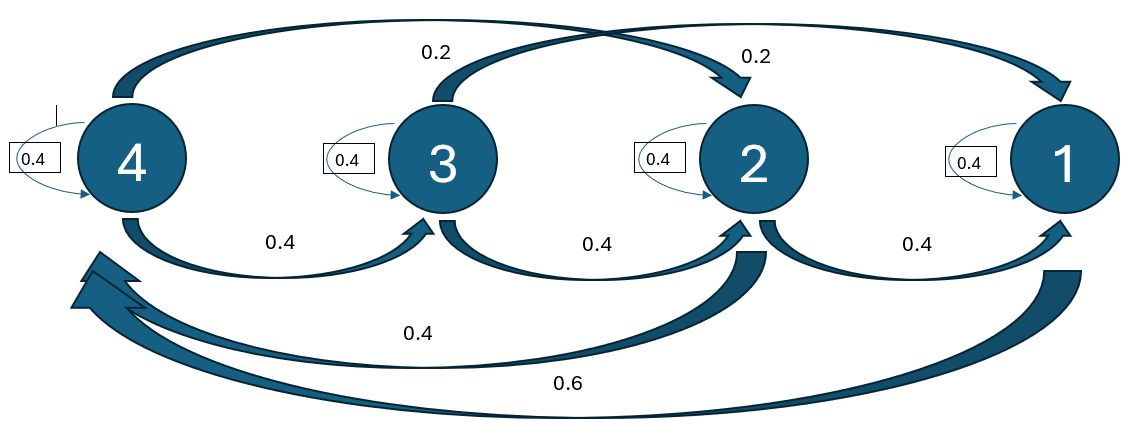
\includegraphics[width=\textwidth]{stat2003_q4a.png} \\

\sol(b) \\
The limiting distribution, $\boldsymbol{\pi}$, if it exists, is a vector such that 
$$
    \boldsymbol{\pi} = \boldsymbol{\pi}P,\quad \sum_{\forall i}\pi_i = 1 \text{ and } \pi_i\geq 0,\ \forall i
$$
Let $\boldsymbol{\pi} = \bracks{\pi_1, \pi_2, \pi_3, \pi_4}$. Then
$$
    \begin{array}{lcl}
         \pi_1 &=& 0.4\pi_1 + 0.4\pi_2 + 0.2\pi_3   \\
         \pi_2 &=& 0.4\pi_2 + 0.4\pi_3 + 0.2\pi_4   \\
         \pi_3 &=& 0.4\pi_3 + 0.4\pi_4    \\
         1 &=& \pi_1 + \pi_2 + \pi_3 + \pi_4   \\
    \end{array}
$$
is a solvable system of linear equations. From WolframAlpha, I find a potential solution,
$$
    \boldsymbol{\pi} = \bracks{\frac{10}{43}, \frac{21}{86}, \frac{9}{43}, \frac{27}{86}}
$$
Just as a sanity check, we can throw these entries into the ``secret'' fifth equation,
$$
    \pi_4 = 0.6\pi_1 + 0.2\pi_2 + 0.4\pi_4 = 0.6\frac{10}{43} + 0.2\frac{21}{86} + 0.4\frac{27}{86} = \frac{27}{86}
$$
as expected. \\
Therefore, In the long run, when the shop opens
\begin{itemize}
    \item ~23\% of mornings begin with 1 racket on the shelf,
    \item ~24\% with 2 rackets,
    \item ~21\% with 3 rackets,
    \item ~31\% with the shelf freshly refilled to 4 rackets.
\end{itemize}

\sol(c)\\
If the start of day stock is 4 or 3, it is impossible to get a restock order. \\
If the start of day stock is 2, there is a 0.2 probability that a restock order is made (the case that 2 rackets are sold). \\
If the start of the day stock is 1, there is a 0.4+0.2 probability that a restock order is made (either 1 racket is sold, or 2 rackets are sold.) \\
$$
    \text{Hence,\ } R(i) := \prob{\text{restock order made}\given \text{morning stock}=i} = \begin{cases}
        \frac{3}{5}, &\ i=1 \\
        \frac{1}{5}, &\ i=2 \\
        0,           &\ i=3,4 \\
    \end{cases}
$$
Then, the long run average,
\begin{align*}
    \expect R &= \sum_{i=1}^{4} \pi_i R(i) \\
        &= \pi_1\bracks{\frac{3}{5}} + \pi_2\bracks{\frac{1}{5}} + \pi_3\bracks{0} + \pi_4\bracks{0} \\
        &= \frac{10}{43}\bracks{\frac{3}{5}} + \frac{21}{86}\bracks{\frac{1}{5}} \\
        &= \frac{30}{215} + \frac{21}{430} = \frac{81}{430} \approx 0.1884
\end{align*}
So, the store expects to restock 0.19 times per day, or once every 5.3 days. \\

\sol(d)\\
A lost sale occurs on days when we start with 1 stock in the morning, and we have two customers. This is the only configuration which results in a lost sale.\\
The probability that We have morning stock of 1 is $\pi_1 = \frac{10}{43}$. \\
The probability that we have 2 customers is always $\frac{1}{5}$, given in the question. \\
Therefore, the expected number of lost sales per day is
$$
    \expect \text{loss}/\text{day} = \frac{10}{43}\cd\frac{1}{5} = \frac{10}{215} \approx 0.0465.
$$

\sol(e)
\begin{verbatim}
[ 1] import numpy as np
[ 2] import pandas as pd
[ 3] 
[ 4] # Parameters
[ 5] days = 1000
[ 6] P = 10
[ 7] C = 15
[ 8] maxStock = 4
[ 9] demandOptions = [0, 1, 2]
[10] demandPr = [0.4, 0.4, 0.2]
[11] 
[12] def simulate(restockStrat):
[13]   stock = maxStock
[14]   restocks = 0
[15]   lostSales = 0
[16]   profit = 0
[17] 
[18]   for _ in range(days):
[19]     demandToday = np.random.choice(demandOptions, p=demandPr)
[20]     if demandToday > stock:
[21]       lostSales += demandToday - stock
[22]       demandToday = stock
[23]         
[24]     stock -= demandToday
[25]     profit += demandToday * P
[26] 
[27]     # Restocking Strategies
[28]     if restockStrat == "zero" and stock == 0:
[29]       stock = maxStock
[30]       restocks += 1
[31]       profit -= C
[32]     elif restockStrat == "less_than_two" and stock < 2:
[33]       stock = maxStock
[34]       restocks += 1
[35]       profit -= C
[36]     else:
[37]       ValueError(f"Unknown strategy: '{restockStrat}'")
[38] 
[39]   return restocks, lostSales, profit
[40] 
[41] # Run both strategies
[42] results = {
[43]   "Strategy": [],
[44]   "Avg Restocks": [],
[45]   "Avg Lost Sales": [],
[46]   "Avg Profit": []
[47] }
[48] 
[49] for strategy_name in ["zero", "less_than_two"]:
[50]   restocks, lost_sales, profit = simulate(strategy_name)
[51]   results["Strategy"].append(strategy_name)
[52]   results["Avg Restocks"].append(restocks)
[53]   results["Avg Lost Sales"].append(lost_sales)
[54]   results["Avg Profit"].append(profit)
[55] 
[56] # Print my results nicely
[57] print(pd.DataFrame(results))
[58] 
\end{verbatim}
\verb|Output:|\\
\verb|            Strategy  Avg Restocks  Avg Lost Sales  Avg Profit|\\
\verb|    0           zero           185              42        4625|\\
\verb|    1  less_than_two           236               0        4170|\\

In conclusion, the ``\texttt{less\_than\_two}'' strategy will result in no lost sales, however the cost of so many additional restocks seriously eats into our profit.


\newpage
\qs{10 marks}{
  A smart irrigation system manages water delivery using the following components:
  \begin{itemize}
    \item two soil moisture sensors (Sensor A and Sensor B) monitors moisture levels.
    \item a central decision unit processes sensor data and determines when irrigation is needed.
    \item two electronic irrigation valves (Valve A and Valve B) which open if instructed.
    \item a power controller provides energy to all components.
  \end{itemize}
  The system is considered operational if both the power controller and the central decision unit are working, and at least one sensor is working, and at least one valve is working.
  \begin{enumerate}[label=(\alph*)]
    \item Draw a block diagram that represents the system's components and their relationships.
    \item Give the structure function for this system.
    \item Assume all six components fail independently and have exponentially distributed lifetimes with mean $\lm$ years. What is the probability that the system is working at some time $t > 0$?
  \end{enumerate}
}
\sol(a)\\
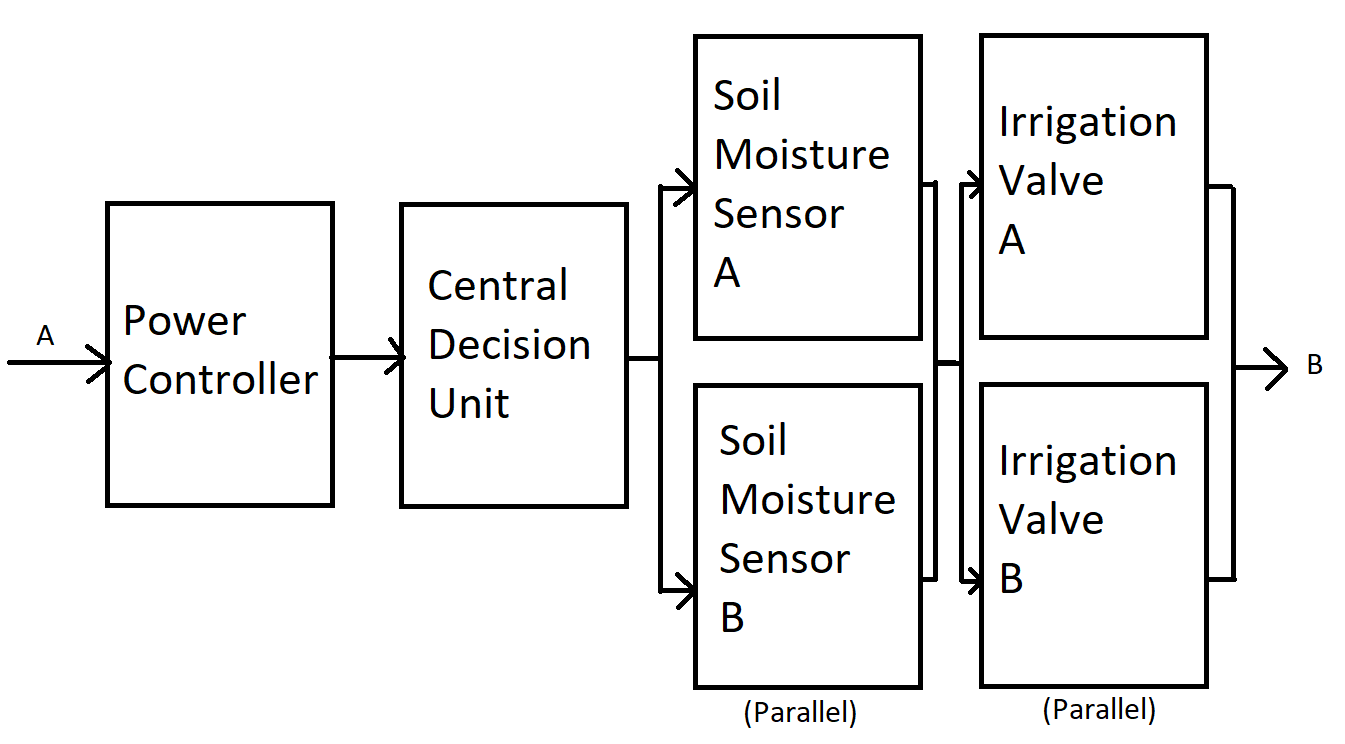
\includegraphics[width=\textwidth]{stat2003_q5a.png} \\

\sol(b) \\
Let $U$ be the set of all my components. \\
$\forall u\in U,\ u=1$ if it is operational, and $u=0$ if it is not. \\
Let $p:=\text{State of Power Controller}$.\\
Let $c:=\text{State of Central Decision Unit}$.\\
Let $s_i:=\text{State of Soil Moisture Sensor}\ i,\ i\in\braces{A,B}$.\\
Let $v_i:=\text{State of Irrigation Valve}\ i,\ i\in\braces{A,B}$.\\

The system, $\phi: U\to\braces{0,1}$, is operational if $p=1$, $c=1$, at least one of $s_A,s_B=1$, and at least one of $v_A, v_B=1$, all in series. In logic, we might express,
$$
    \phi \equiv p\land c\land (s_A \vee s_B) \land (v_A \vee v_B)
$$
The structure function is given by
\begin{align*}
    \phi(u) = \phi(p,c,s_A,s_B,v_a,v_b) &= pc(1 - (1-s_A)(1-s_B))(1 - (1-v_A)(1-v_B)) \\
        &= pc(s_A + s_B - s_As_B)(v_A + v_B - v_Av_B)     
\end{align*}

\sol(c) \\
Let $r(t):=\text{Be the probability the component is still operational at time}\ t$. We are given that $r(t) = e^{-t/\lm}$. \\
$p$ is in series, so it's reliability $r(t)$. \\
$c$ is in series, so it's reliability $r(t)$. \\
$s_i$ is in series, so it's reliability is multiplied. \\
$v_i$ is in series, so it's reliability is multiplied. \\
However, $s_A$ and $s_B$ are in parallel, so we need to apply the formula,
$$
    r(s) = 1 - \prod_{i\in\braces{A,B}} (1-r(t)) = 1 - (1-r(t))(1-r(t)) = r(t)(2 - r(t))
$$
$v_A$ and $v_B$ are similarly parallel, and their $r$ is similarly expressed,
$$
    r(v) = r(t)(2-r(t))
$$
The overall reliability then is given by
$$
    R(t) = r(t) r(t) r(t)(2-r(t)) r(t)(2-r(t)) = r(t)^4(2-r(t))^2 = e^{-4t/\lm}(2-e^{-t/\lm})^2
$$
and represnets the probability that the entire system is operational at time $t$.


\end{document}
